\chapter{Theory\label{ch:theory}}
\section{Recombination X-Ray Laser}
\subsection{The overall processes}
The overall processes, could be divided into three stages, ionization,
cooling and expansion, recombination and gain.

When the laser fields are applied, due to its Gaussian distribution,
initial field is weak, but increasing rapidly. As long as the
tunneling ionization threshold is reached, the ionization will be
finished instantly.

The dominating ionization mechanism is optical field ionization.

When the laser passed away, the left process is cooling and expansion.
During this stage, the total energy of the system is decreasing, so it
is called cooling. During these processes, the electron density
distribution is still altering due to the collisions between different
particles, like electron-electron, ion-ion, and electron-ion. Another
effect brought by those collision is the plasma expansion, whose speed
is around $10^6$cm/s. But since the total period for cooling and
expansion is as short as $1ps$, the expansion($1ps*10^6cm/s=0.01\mu
m$) is not that dramatic.


\subsection{All the processes, like 3-body Recombination}
\subsection{Tunnelling ionization}
When the energy of laser is relatively small, and the duration of the
pulse is as long as nanosecond, the ionization could be avalance, for
during this nanosecond period, multiple collision is possible.

Then if the energy of laser pulse is increased, multi-phone ionization
process becomes to show up.

By incrementing the energy further, to the point when the electric
field in the laser beam reach the level comparable to the electric
field inside the atoms (around $10^9 V/m$), then the external laser
field is strong enough to get the Columb field of atoms suppressed,
which is called tunneling ionization. The tunneling rate is increased
dramatically during tunneling ionization process.

TODO: Yoav talk's picture.

The timescale of tunneling ionization could be considered as completed
instantly, actually it's around 10 to several hundreds
atto-second. Usually we treat timescales lower than 1 femto-second to
be instantly done.

\subsection{Heating mechanism}
The processes of both ionization and heating evolve
simultaneously. The main heating mechanism is residual heating, which
is mainly due to the phase lag between electrons and laser field.

The other heating mechanism is collision. But this effect may be neglected.
For collisional heating exists only when Laser is
present. Intuitively, it's similar to cooking, when the laser passed
away, it's like the cooking fire is gone, so there's no collional
heating any more. However, since the laser only last for tens
femtosecond, during this so-short period, the particles have no enough
time to colloid with each other, so actually the collisional heating
could be neglected.

\subsection{Recombination and gain}
This process depends on the lifetime of the excited states, it is
small as well, for example the Carbon 2->1 lifetime is 1.4ps
only. After this period, all the population will be back to ground
state, nothing happens.

\section{LWI}
\begin{figure}[htb]
  \begin{center}
    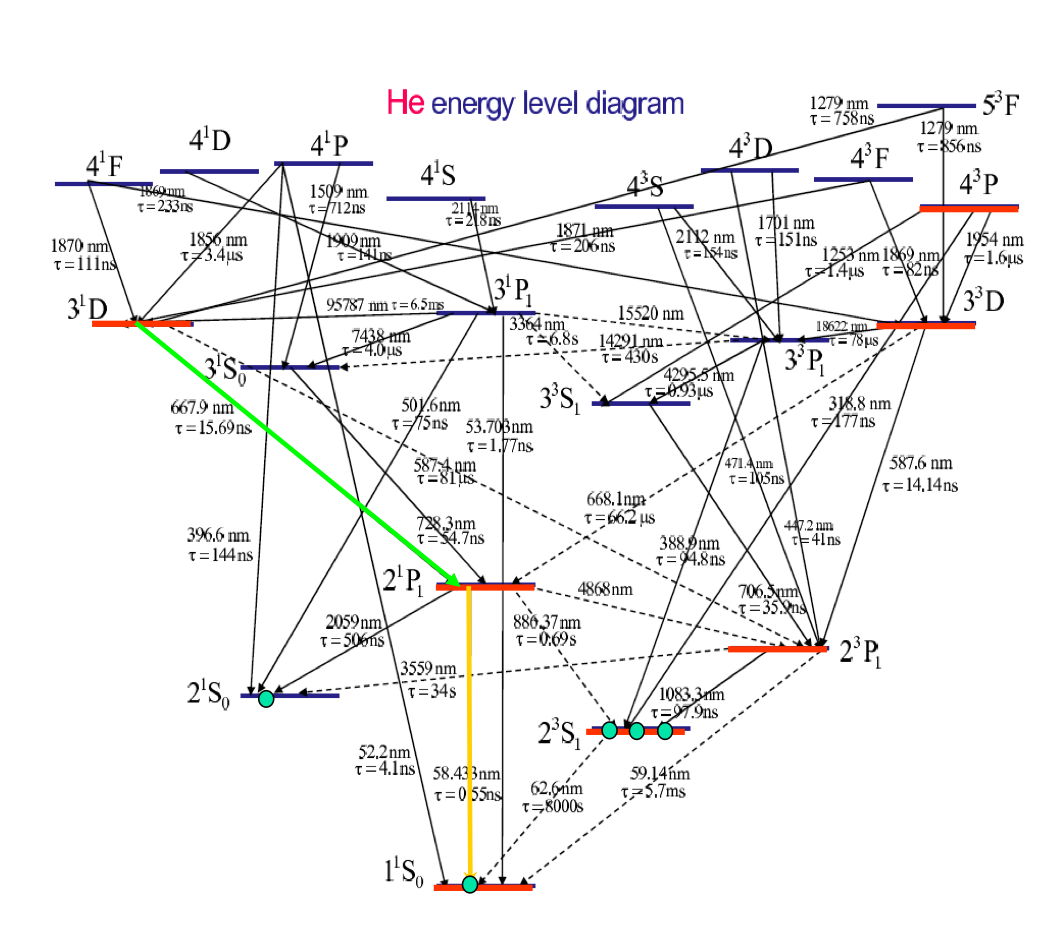
\includegraphics[width=0.9\linewidth]{ch-theory/figures/Helium_energy_levels}
    \caption[Sample Title Page Layout]{Helium energy levels~\cite{drake2007multiplet}}
    \label{fig:theory:HeEnergyLevel}
  \end{center}
\end{figure}


